\documentclass[notitlepage]{report}
\usepackage{graphicx}
\usepackage[left=1in, right=1in, top=1in, bottom=1in]{geometry}
\usepackage{titling}
\usepackage{lipsum}
\pretitle{\begin{center}\Huge\bfseries}
\posttitle{\par\end{center}\vskip 0.5em}
\preauthor{\begin{center}\Large\ttfamily}
\postauthor{\end{center}}
%\predate{\par\large\centering}
%\postdate{\par}
\usepackage{natbib}

\title{Bibliometrics and DFT}
\author{Us and others}
%\date{\today}
\date{}
\usepackage{color}
\begin{document}
\maketitle
\thispagestyle{empty}
Sir:\\

In this Viewpoint, we extend the bibliometric technique of co-citation to generate citation statistics that illustrate the history of the popular B3LYP model.


When two articles are cited by a third one for the first time, two previously existing ideas are combined into a new one. This pattern is referred to as co-citation, and its frequency, which accumulates over time, represents the extent to which this idea is recognized by the research community. Co-citation was independently described by Marshakova-Shaikevich and Small in 1973~\citep{MarshakovaShaikevich1973,Small1973} and co-citation measurements have since been extensively used in scientometrics. 

From a sampling of the physics literature, Small reported 4 pairs of articles with a co-citation frequency of 49 and greater (ibid). This was in 1973 but the volume of scientific literature has since grown considerably; more co-cited pairs have been discovered, citation frequencies have increased, as well as the scale of bibliometric studies. Improved bibliographies and modern computing tools have also rendered co-citation calculations relatively facile and co-citation has been measured over tens of millions of articles, and the high end of co-citation frequencies is in the tens of thousands~\citep{Stringer2010,Uzzi2013,devarakonda_2020}

A natural extension of co-citation theory is document coupling of a higher order, for example, triads and tetrads that are correspondingly tri-cited and tetra-cited. Another way of looking at these patterns is to view any article $A$ that cites $n$ articles as comprising $n$ citations, $n\choose2$ co-citations, $n\choose3$ tri-citations etc. Calculating the frequencies of these combinations in a bibliography is relatively expensive and may have dissuaded such investigation. For example, an article with either 25 or 50 cited references represents 300 or 1,225 co-citations respectively. The same article also consists of  2,300 or 19,600 tri-citations and  12,650 or  230,300 tetra-citations. For even a modestly sized collection of 2 million articles with an average of 30 references each, this could involve computing $8.12\times10^9$ tri-citations, $5.48\times10^{10}$ tetra-citations, or $2.85\times10^{11}$ penta-citations. Scalable and affordable computing today places measuring these higher order assemblies within reach of the scientometrist, and may open a frontier for discovery that extends beyond co-citation.

Small proposed a model of multiple citation in 1974~\citep{small1974multiple} in which an example of tri-citations measured over a set of 6 publications was presented. In an initial exploration of higher-order combinations, we have used a `brute force' approach to compute triad fquencies from an 11-year dataset of articles in the Scopus bibliography to identify 181 million triads that have been tri-cited upto 13,000 times since publication. Much like citations and co-citations, the vast majority of tri-citations are of very low frequency suggesting modest community recognition. High frequency triplets naturally pique interest. 

\begin{figure}[h!]
\begin{center}
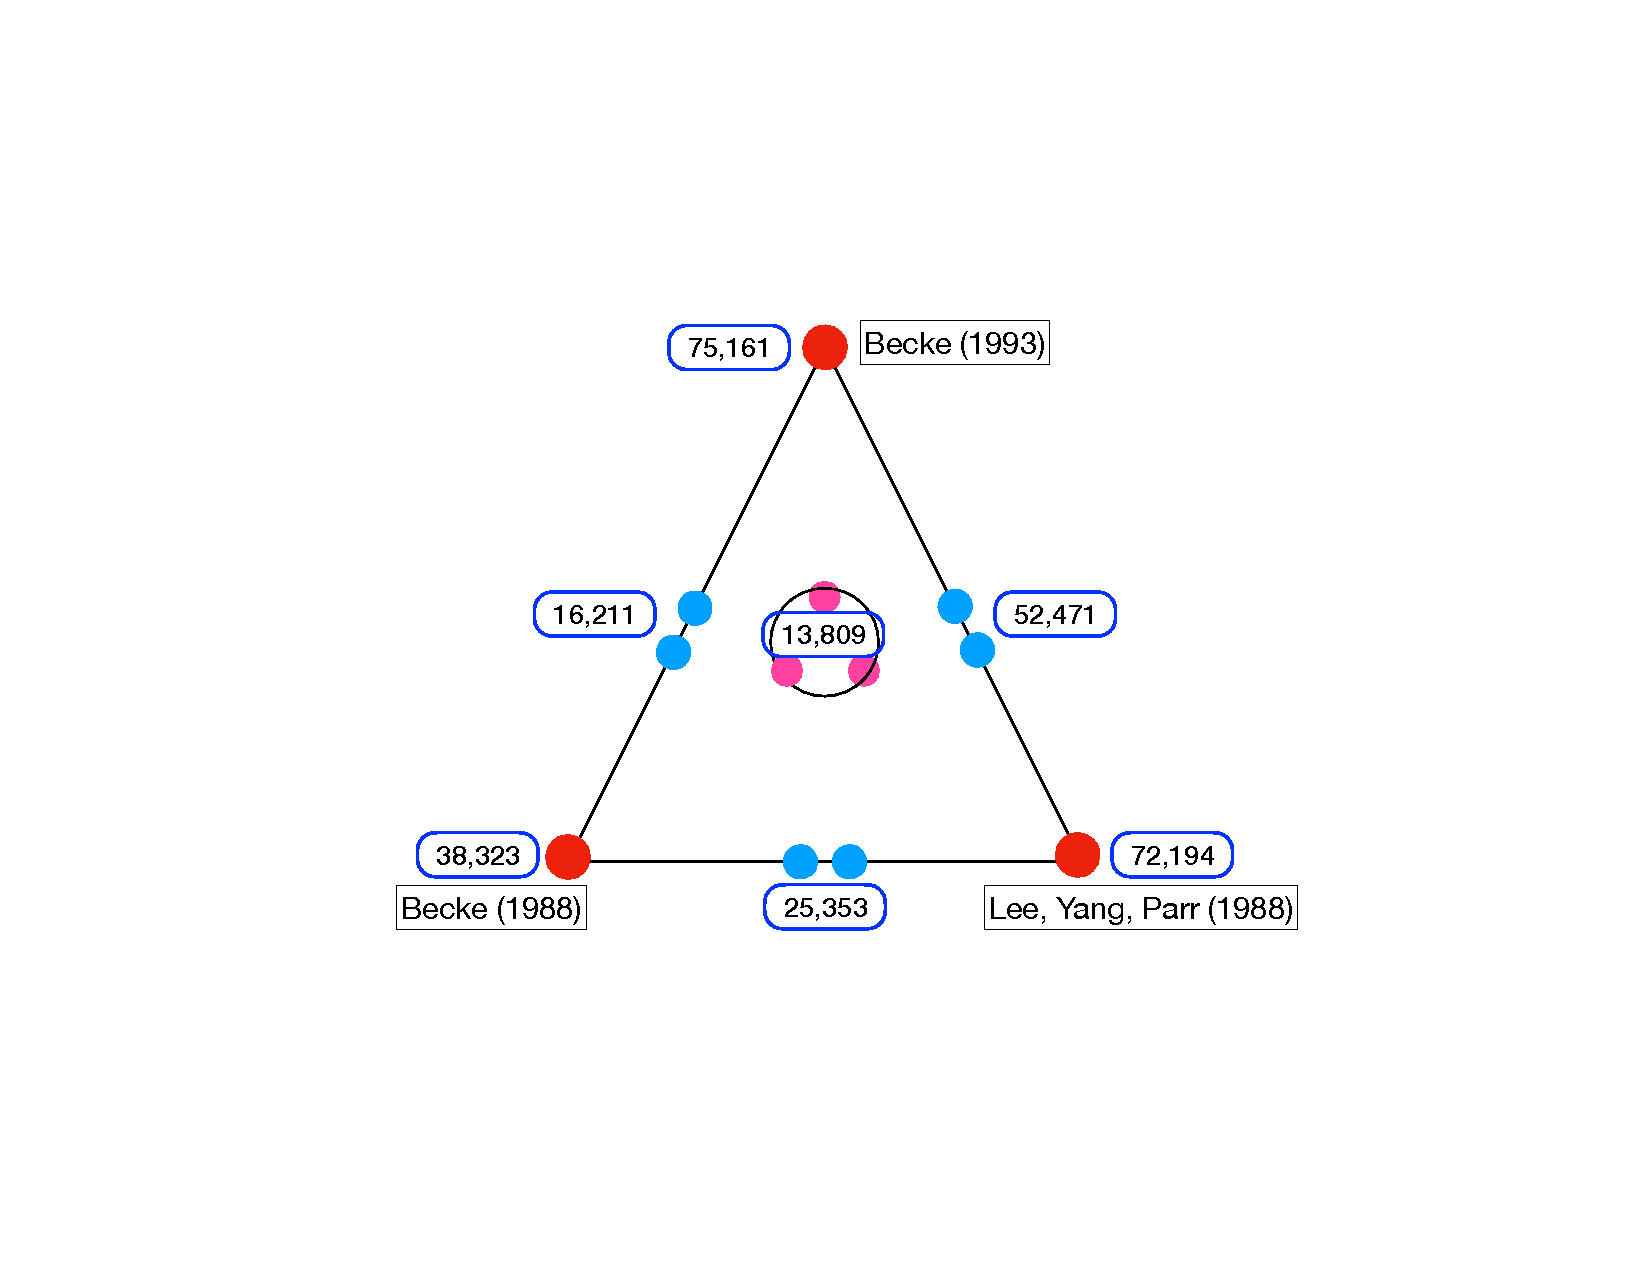
\includegraphics[width=10cm]{fig1.pdf}% This is a *.eps file
\end{center}
\caption{A high frequency triplet. The triad of (i) Becke (1988), (ii) Becke (1992), and (iii) Lee, Yang, and Parr (1988).  Frequencies (round rectangles with blue borders) are shown for the tri-citation (center of triangle), co-citations (sides of triangle), and 
article citations (vertices of triangle). 
}
\label{fig:fig1}
\end{figure}
The triad with the highest frequency that we observed in 181 million cases is tri-cited 13,000 times.  All three elements of the triad originate in density functional theory (DFT). The first citation of this triad likely arose because of a paper published by Stephens, Chabalowski, Devlin, and Frisch~\citep{stephens1994ab} in 1994, which blended these Exchange and Correlation functionals into a method called B3LYP (Becke-3 Exchange and Lee-Yang-Parr Correlation). In the B3LYP model, two functionals of the electron density are needed. One is the Exchange functional (two electrons of the same spin cannot be at the same point in space) and the other is the Correlation functional (accounting for the correlated motion of electrons with the same spin). The B3LYP method had a lot of advantages in terms of speed and accuracy for the study of organic molecules especially and was rapidly taken up by the computational chemistry and organic chemistry communities.

Historically, B3LYP originates from an effort in the 1908s to to build Exchange and Correlation functionals to allow for the practical application of DFT to chemical problems. A number of groups were engaged and the Becke group in its 1988 and 1993 papers developed an Exchange functional~\citep{becke1988density,becke1993dft}, while Lee, Yang, and Parr (LYP) developed a Correlation functional in their 1988 paper~\citep{lyp1988}. This major advance can be concisely referenced by citing Becke (1988), LYP (1988) and Becke (1993) since the two Becke articles provide the Exchange functional and the Lee-Yang-Parr article contributes with the Correlation functional. The high frequency of co-citation (52,000) of Becke-1993~\citep{becke1993dft} and LYP-1988~\citep{lyp1988} may result from authors assuming that citing Becke's 1993 article is adequate to reference the Exchange functional. 

The three article pairs in the Becke (1988), LYP (1988), Becke (1993) triad have also been co-cited as pairs 16,000, 25,000, and 52,000 times, and the individual articles have been cited 38,000, 72,000, and 75,000 times respectively (Figure 1) \footnote{Citation frequencies vary according to the bibliographic source used so all frequencies reported have been rounded down to the nearest thousand.}. It is more difficult to conjecture why these three articles are individually cited at much higher levels although it is worth noting that  frequencies of article citations always exceed those of co-citations, which in turn exceed those of tri-citations. It is very likely that these articles individually stimulated new ideas although careless citation practice cannot be ruled out entirely.

An interesting community discussion thread~\citep{johansson2002} provides the opinion that a complete set of citations for B3LYP is (i) Vosko, Wilk and Nusair (1980)~\citep{vosko1980accurate} (ii) Becke (1988) (iii) LYP (1988) (iv) Becke (1993) (v) Stephens 1994. It is interesting to note that Stephens, Chabalowski, and Frisch cite Vosko, Wilk and Nusair (1980), which is not cited in Becke (1988), Becke (1993), or LYP (1993). 

We emphasize that citations always tell only a part of the story but are quite valuable in tracing history and estimating impact. In this case, the triad leads us to a cluster of publications that are associated with a major advance in applying DFT to practical use (Kennie needs to approve or rewrite my hand waving). Examining the three component co-cited pairs of the triad allows us to infer that Becke (1993) and LYP (1988) are most extensively recognized 
in the community as far as B3LYP is concerned. 

\bibliographystyle{acm}
\bibliography{B3LYP}

\end{document}